To run the experiments in this paper, we used a DDD pacemaker model developed according to the specification derived from the Boston Scientific Challenge~\cite{challenge}.
\todo[inline]{ZJ : 2-3 lines describing the PM model.}

More information about the implementation can be found in \cite{testing}. 

%\textbf{1. Lower Rate Interval (LRI)}:
%The LRI interval starts at a ventricular sensed or paced event. The LRI interval is the longest interval between two ventricular events. 
%
%\textbf{2. Upper Rate Interval (URI)}:
%The URI interval defines the shortest interval between a ventricular event and a paced ventricular event
%
%\textbf{3. Atrial-Ventricular Interval (AVI)}:
%Ventricular pacing shall occur in the absence of a sensed ventricular event within the programmed AV delay when the time elapsed after the last ventricular event is between the programmed LRI and URI.
%
%\textbf{4. Ventricular Refractory Period (VRP)}:
%The VRP is the time interval following a ventricular event during which no ventricular sense (VS) can happen.
%
%\textbf{5. Post Ventricular Atrial Refractory Period (PVARP)}:
%The PVARP is the time interval following a ventricular event during which no atrial sense (AS) can happen.
%
%According to the five primary specifications of the basic DDD pacemaker, a Simulink model was designed using temporal logic. Each component corresponds to a particular specification and communicates with others using channels. A timing diagram is shown in \ref{timingPM}. 
%%%%%%%%%%%%%%%%%%%%%%%%%%%%%%%%%%%%%%%%%%%%%%%
%\begin{figure}[!b]
%	\center
%	\vspace{-10pt}
%	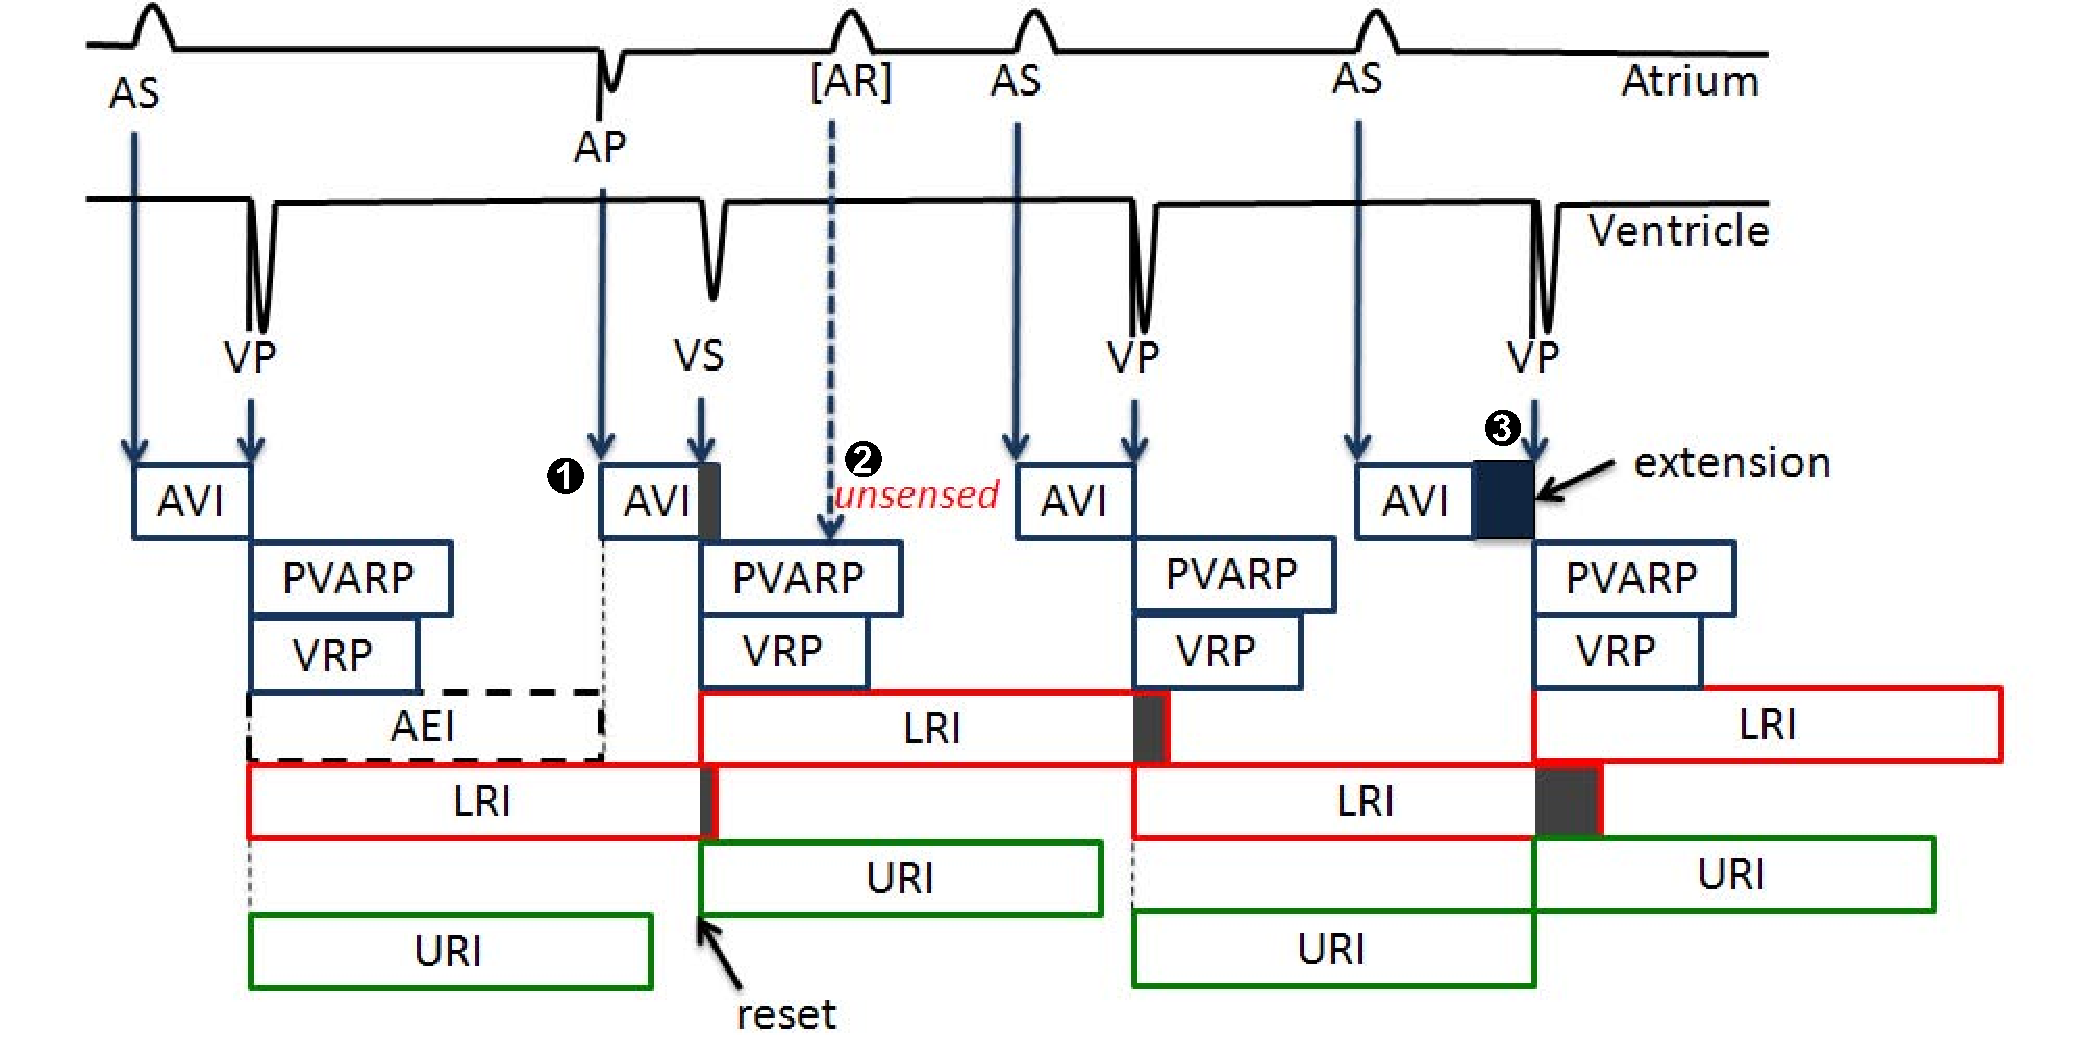
\includegraphics[width=0.45\textwidth]{figures/PM_timers.pdf}
%	\vspace{-10pt}
%	\caption{Simulink design of path automata}
%	\label{fig:timingPM}
%\end{figure}